\documentclass[12pt]{article}

% PACKAGES

\usepackage{hyperref}
\usepackage{graphicx}
\graphicspath{ {./images/} }

% CUSTOM COMMANDS

\newcommand{\row}[1]{\texttt{#1}}
\newcommand{\br}[0]{\vspace{10pt} \noindent}
\newcommand{\footurl}[1]{\footnote{\url{#1}}}
\newcommand{\nth}[2]{#1\textsuperscript{#2}}

% TITLE

\title{Insert Report Title Here}
\author{Benjamin White-Horne \\ \emph{Oxford University}}



\begin{document}

\maketitle



\pagebreak

\section*{Abstract}

This project concerns the designing and prototyping of Jigsaw, an application to help change ringing
composers to compose while requiring as little change to their workflow as possible.  In other
words, Jigsaw aims to be to composers is to Microsoft Word is to writers.  Additionally, I hope that
the addition of a beginner-friendly visual tool will make composing easier for people to get into
(MU/DA:\@ please reword this --- thanks).  Jigsaw is currently deployed as a static web app using
GitHub pages.

Whilst writing Jigsaw I also created BellFrame, a fast and idiomatic Rust library which provides
easy-to-use datatypes for ubiquitous concepts in change ringing.  BellFrame has good documentation
with code examples, and is in itself a very useful asset.  Once its API is more stable, I will
publish it to Rust's package repository for general use.

\br{}Change ringing is an art form which is almost exclusive to England, where people ring sets of
bells in continually evolving sequences, known as `changes' or `rows'.  The art of `composing'
concerns designing sequences of rows for ringers to perform, and predates computers by several
centuries (the ealiest surviving record of composing come from Fabian Stedman in the 1700s).

Compositions are at their core sequences of permutations and are therefore extremely ameanable to
both mathematical and computer analysis.  Some parts of composition have already been well
automated, including brute-force generation of compositions, but there are very few user-friendly
tools for composers.  By prototyping Jigsaw, I have explored one possible way to fill this gap.



\pagebreak

\tableofcontents



\pagebreak

\section{Introduction}

\subsection{Change Ringing and Composing}

\subsection{Project Goals}

This project concerns prototyping an application to \emph{aid} composers whilst requiring the
smallest possible change to their existing workflow.  This is analogous to what Microsoft Word
provides for writers --- a kind of `automated paper' which automatically annotates your work with
data that is tedious to compute manually whilst still providing it in a format that you are familiar
with (i.e.\ words on a page).  Additionally, it must provide correct feedback regardless of the
completeness of the composition.

Whilst this goal is good for general direction, we need more specific goals in order to build a
cohesive application.  Therefore, I will split up this general goal into simpler goals which can
easily be used to rate the resulting application.  Most of these come from observations of existing
programs, conversations with well-known composers, and experience gained from experimentation early
in the project.

\paragraph{Ease of Use} The application should be made so that anyone can install and use it easily,
without any technological knowledge or a lengthy installation process.

\paragraph{Completeness} There is a concrete definition of what is considered `Change
Ringing'\footnote{The definition is defined by the Framework for Method Ringing, found here:
\url{https://cccbr.github.io/method_ringing_framework/classification.html}}, and the states
representable in the application must be a superset of this definition.

\paragraph{Incremental} The application should allow the user to incrementally build up their
composition, in whatever order they want, starting wherever they want to.  Specifically, it must
be able to represent `partial' compositions --- i.e.\ a set of composition `fragments' which will
eventually be combined into a full composition.

\paragraph{Instant} Feedback on important measures like truth, music content and length should
always update instantly whenever the composer changes their composition.

\paragraph{Visual} Everything that can be understood visually should be displayed visually.  Where
concrete numbers are required (e.g.\ length), these should also be provided.

\subsection{Jigsaw}

\subsubsection{Static Web Application}

\subsubsection{Rust and WebAssembly}

\subsubsection{BellFrame}

\subsubsection{Code Architecture}



\pagebreak

\section{Overview of Change Ringing}

\subsection{\ldots}



\section{Implementation}

\subsection{Model-View-Presenter}

\subsection{Undo History}

\subsection{Specification vs Derived State}

\subsection{BellFrame}



\pagebreak

\section{Conclusion}

This project has two major products: the application itself (named Jigsaw) and the reusable utility
library on which Jigsaw is built (named BellFrame).

As it stands right now, I think that BellFrame is a bigger contribution to composing (despite
technically being a bi-product) since it is very usable and has some battle-testing.  Jigsaw, on
the other hand, is a very promising prototype but is not feature complete or stable enough to be
used in production.  Fixing both these issues is simply a matter of development time and testing, 
and I will continue working on Jigsaw even after this project is handed in.  Given the limited
time-frame of this project, I chose to spend it on exploring unexplored ideas rather than striving
for perfect stability.

\subsection{Jigsaw}

I think that Jigsaw is a successful prototype and I will likely continue building it into a
feature-complete application.  I demonstrated it to several other composers who all thought it
looked very promising.  It has a number of small rough edges which would make the current iteration
difficult to use in production, but do not detract from its value as a prototype.

In order to decide on the success of the project, I will rank it against the design goals set out in
Section~\ref{sec:design-goals}.

\subsubsection{Ease of Use \& Visual}

Firstly, building Jigsaw as a single static page means it requires no installation to use.  The
design of an infinite canvas plus a folding sidebar feels very natural and intuitive to use.

A large amount of effort went into making sure that GUI is visually crisp and responsive.  This
goes as far as rounding all coordinates to the nearest pixel to prevent fuzzy boundaries
(screenshot?), as well as doing the same for line rendering --- see
Section~\ref{sec:line-rendering}.  This attention to detail makes the experience of using Jigsaw
feel very smooth and polished.

All actions are currently bound to keyboard shortcuts which means that editing compositions quickly
becomes muscle memory for experienced users, but feels unintuitive to beginners since at any point
in time there's no indicator of what actions are available.  If I had more time, I would add a
contextual right-click menu to fix this problem (it could even show the key bindings to help
beginners learn them).

\subsubsection{Completeness}

Jigsaw's internal representation is complete, but the current user interface is not.  In other
words, Jigsaw is internally able to represent a strict superset of compositions which are considered
change ringing, but the prototype GUI means that the user is unable to express some very obscure
states which are technically considered change ringing.  For perhaps 99\% of use cases, Jigsaw's
user interface is complete enough that most users would not notice.

\subsubsection{Incremental}

Jigsaw is completely built around being incremental.  It also does its best to preserve `continuity'
of operations --- that is, a small operation should cause a small change to the composition's rows.
Some operations like splitting and joining fragments only change the structure of the composition,
and not the output rows.

\subsubsection{Instant}

Due to the internal architecture, the composition is always fully annotated.  Whenever the user
causes an update, the entire state of the display is recalculated then cached for repainting.
Therefore, it simply isn't possible for any part of the changes to lag behind because the full UI
state is simultaneously recalculated after every change.

This does, however, mean that Jigsaw is extremely dependent on the efficiency of this update
pipeline.  Luckily, Rust and WebAssembly seem to be working extremely well here since the pipeline
is fast enough to reliably feel instant, even for extremely large compositions.  I haven't done any
specific optimisations, but I have also been mindful of high-level performance when writing the code
--- the algorithms are all $O(n \log n)$ in the number of bells in the composition, although the
link detection is $O(n^2)$ in the number of fragments.

Whilst stress testing Jigsaw, I discovered that this delay becomes noticeable at around 35,000
$\times$ 8 = 280,000 bells (see Figure~\ref{fig:stress-test}).  Since at least 99.9\% of
compositions have at most 10,000 rows each of 16 bells (making 160,000 bells total) I think that the
performance is perfectly adequate.

The longest piece of ringing ever rung contains 72,000 $\times$ 6 = 432,000 bells, which would cause
the current implementation some consternation.  In reality, the composition for this was split into
many separate pieces to ease memorability so I doubt anyone would want to reason about the
composition in full.  However, I would like Jigsaw to eventually support huge compositions, and
there is plenty of low hanging fruit left to optimise --- for example, the pipeline does no caching
or re-use of memory allocations so the code generates huge numbers of needless allocations during
each pipeline run.

Lastly, BellFrame contains the \verb|SimdRow| type which uses SIMD instructions
(specifically \verb|pshufb|) to perform row permutations in a single clock cycle, which usually
increases performance by at least an order of magnitude.  However, SIMD support in WebAssembly is
not mainstream yet so Jigsaw can't take advantage of this.

\begin{figure}
    \centering
    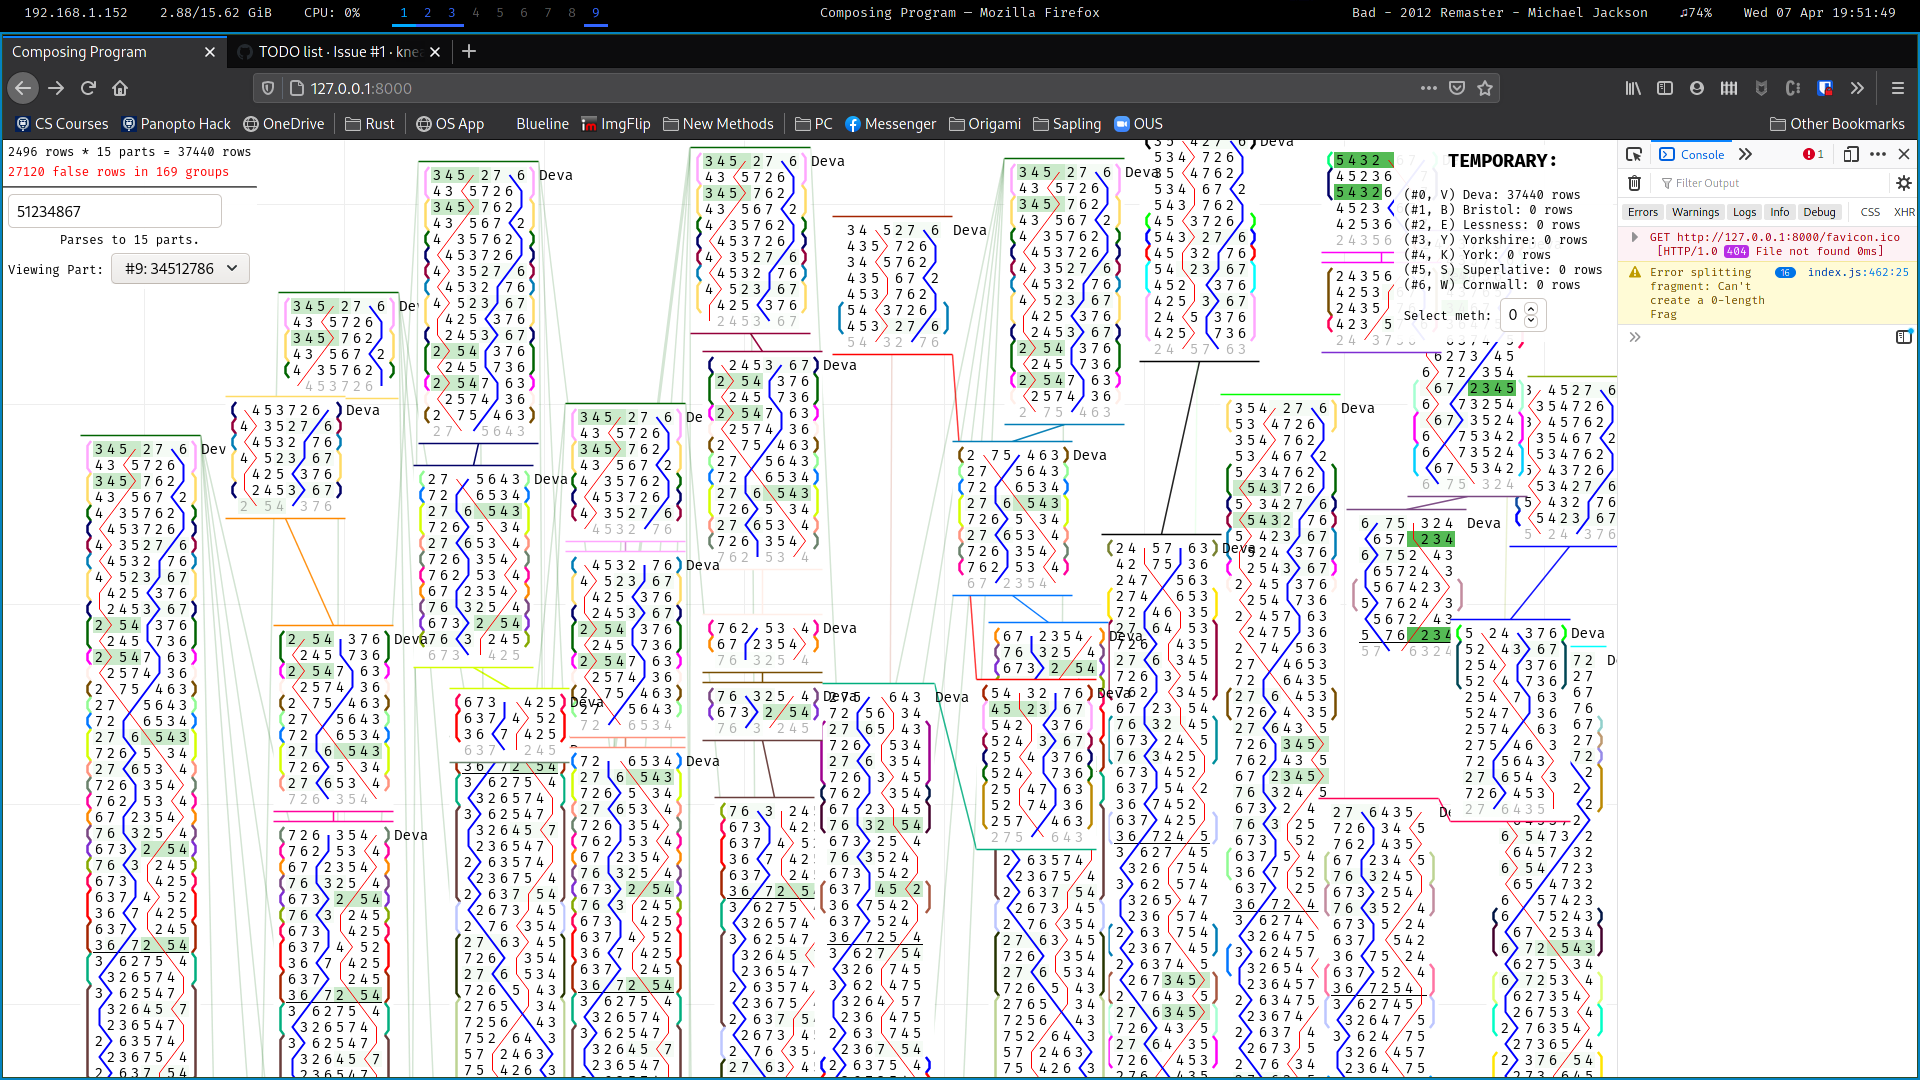
\includegraphics[width=\textwidth]{stress-test}
    \caption{Stress testing Jigsaw (the GUI has since changed, but the pipeline has
    not).}\label{fig:stress-test}
\end{figure}



\pagebreak

\section{Glossary of Change Ringing Terms}

\paragraph{Stage:} The number of bells which the composition uses.  This is not necessarily the
number of bells used to ring a given composition, but for the purposes of this project the
distinction is not relevant.

\paragraph{Row:} A sequence of bells which forms a permutation.  Rows are the fundamental building
blocks of compositions.  The words `change' and `row' are often used interchangeably (hence the name
`Change Ringing'), but to avoid confusion I will always use `row' in this report.

\paragraph{Composition:} An ordered sequence of rows which tell ringers in which order the bells
should be rung.

\paragraph{Truth:} For the purposes of this project, a composition is \emph{`true'} if all the rows
are unique, otherwise it is \emph{`false'}.  This is the single most important property of a
composition, since any performance of a `false' composition is considered invalid.

\paragraph{Method:} A short, usually symmetrical, pattern that is repeated throughout a composition
with small and well-defined modifications (known as `calls').  This is the key to how human ringers
can ring over 5000 rows worth of composition without any memory aid --- in reality, they memorise
the method(s) and one `conductor' memorises the pattern of calls and calls them in the right places
for the other ringers to take effect.  It is usually the job of the composer to make sure that the
call sequence is predictable and easy to memorise.

\paragraph{Lead:} A single instance of the repeating pattern of a method.

\end{document}
